\documentclass[11pt]{article}

\usepackage[headheight=14pt,a4paper]{geometry}
\geometry{left=2.0cm,right=2.0cm,top=2.5cm,bottom=2.5cm}

\usepackage[UTF8]{ctex}
\usepackage{tikz}
\usepackage{tikz-qtree}
\usepackage{pstricks}
\usepackage{amsfonts,graphicx,amssymb,bm,amsthm}
\usepackage{algorithm,algorithmicx}
\usepackage[noend]{algpseudocode}
\usepackage{fancyhdr}
\usepackage[fleqn]{amsmath}
\usepackage{listings}

\newenvironment{solution}{{\noindent\hskip 2em \bf 解 \quad}}

\renewenvironment{proof}{{\noindent\hskip 2em \bf 证明 \quad}}{\hfill$\qed$\par\vskip1em}
\newenvironment{proofs}[1]{{\noindent\hskip 2em \bf #1 \quad}}{\hfill$\qed$\par\vskip1em}

\makeatletter

\let\old@@children\@@children
\def\@@children{\futurelet\my@next\my@@children}
\def\my@@children{%
\ifx\my@next\missing\else
\expandafter\@gobble
\fi
\expandafter\old@@children}

\makeatother

\newcommand{\missing}{ \edge[draw=none]; \node[draw=none]{}; }
\newcommand{\tabincell}[2]{\begin{tabular}{@{}#1@{}}#2\end{tabular}}

\begin{document}

\pagestyle{fancy}
\rhead{\kaishu 数据结构}

\begin{center}
  {\LARGE{\bf{数据结构作业}}}\\
  {\large{\bf{第三次}}}\\
\end{center}

\begin{flushright}
  \begin{kaishu}
    姓名:刘士祺 \\
    学号:2017K8009929046 \\
  \end{kaishu}
\end{flushright}

\begin{enumerate}
  \item[5.] 习题8-1
    \begin{enumerate}
      \item [1)]
        \begin{solution} \\
          \input{8-1-1.tex}
        \end{solution}
      \item [2)]
        \begin{solution} \\
          \input{8-1-2.tex}
        \end{solution}
    \end{enumerate}
    
  \item[6.] 习题8-7

  \item[7.] 习题9-1 \\
    \begin{solution}
      \begin{enumerate}
        \item [1)] 相同
        \item [2)] 不相同
        \item [3)] 不相同
      \end{enumerate}
    \end{solution}
    
  \item[8.] 习题9-14 \\
    \begin{solution}
      建成的树: \\
      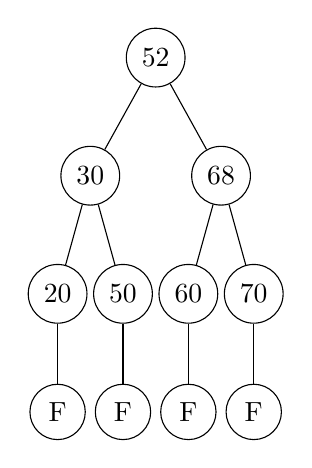
\begin{tikzpicture}
        \tikzset{every tree node/.style={minimum width=2em,draw,circle},
          blank/.style={draw=none},
          edge from parent/.style=
          {draw,edge from parent path={(\tikzparentnode) -- (\tikzchildnode)}},
          level distance=1.5cm}
          \Tree [.52
                  [.30
                    [.20 F ]
                    [.50 F ]]
                  [.68
                    [.60 F ]
                    [.70 F ]]]
      \end{tikzpicture} \\
      删去50: \\
      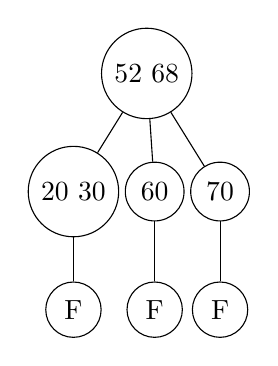
\begin{tikzpicture}
        \tikzset{every tree node/.style={minimum width=2em,draw,circle},
          blank/.style={draw=none},
          edge from parent/.style=
          {draw,edge from parent path={(\tikzparentnode) -- (\tikzchildnode)}},
          level distance=1.5cm}
          \Tree [.52\ 68
                  [.20\ 30 F ]
                  [.60 F ]
                  [.70 F ]]
      \end{tikzpicture} \\
      删去68: \\
      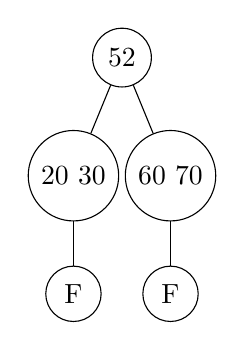
\begin{tikzpicture}
        \tikzset{every tree node/.style={minimum width=2em,draw,circle},
          blank/.style={draw=none},
          edge from parent/.style=
          {draw,edge from parent path={(\tikzparentnode) -- (\tikzchildnode)}},
          level distance=1.5cm}
          \Tree [.52
                  [.20\ 30 F ]
                  [.60\ 70 F ]]
      \end{tikzpicture} \\
    \end{solution}

  \item[9.] 习题9-19 \\
    \begin{solution}
      平均长度为:
      $$\frac{1}{8}(1+1+1+1+2+2+6+3)=\frac{17}{8}$$
    \end{solution}

  \item[10.] 习题9-24

  \item[11.] 习题10-1
    \begin{enumerate}
      \item [1)]
        (087,503,061,512,170,897,275,653,426,908) \\
        (087,061,503,170,512,275,653,426,897,908) \\
        (061,087,170,503,275,512,426,653,897,908) \\
        (061,087,170,275,426,503,512,653,897,908)
      \item [2)]
        (170,087,275,049,426,503,897,512,653,908) \\
        (170,049,275,087,426,503,653,512,897,908) \\
        (049,087,170,275,426,503,512,653,897,908)
      \item [3)]
        (087,061,170,275,426)(503)(512,908,897,653) \\
        (061)(087)(170,275,426)(503)(512)(908,897,653) \\
        (061)(087)(170)(275,426)(503)(512)(897,653)(908) \\
        (061)(087)(170)(275)(426)(503)(512)(653)(897)(908) \\
        (061,087,170,275,426,503,512,653,897,908)
      \item [5)]
        (503)(087)(512)(061)(908)(170)(897)(275)(653)(426) \\
        (503)(087)(512)(061,908)(170)(897)(275)(426,653) \\
        (087,503)(061,512,908)(170,897)(275,426,653) \\
        (061,087,503,512,908)(170,275,426,653,897) \\
        (061,087,170,275,426,503,512,653,897,908)
    \end{enumerate}

  \item[12.] 习题10-3 \\
    \begin{solution}
      堆排序、快速排序、希尔排序是不稳定的排序算法,而基数排序、插入排序、归并排序是稳定的排序算法。 \\
      希尔排序:2,2,1,3 \\
      快速排序:2,1,1,3 \\
    \end{solution}

  \item[13.] 习题10-15

  \item[14.] 习题10-21

  \item[15.] 习题11-1

  \item[16.] 习题11-2

  \item[17.] 习题11-5

  \item[18.] 习题11-11
\end{enumerate}
\end{document}
